\documentclass[10pt,twocolumn]{article}

% This draft is intentionally venue-neutral. Replace the document class and
% margins with the target conference template once the venue is selected.
% Result freeze: 2026-09-11.
% Audited local sources: 4 sep presentation.md, ABLATION.md,
% bch-arc-ct/docs/RETRIEVAL_RESULTS_2026-09-07.md, and metric JSON artifacts.
% The later Biltir handoff should be merged only after matching each value to
% its checkpoint, split, input availability, and inference readout.
\usepackage[margin=0.68in,columnsep=0.22in]{geometry}
\usepackage[T1]{fontenc}
\usepackage{lmodern}
\usepackage{microtype}
\usepackage{booktabs}
\usepackage{multirow}
\usepackage{makecell}
\usepackage{tabularx}
\usepackage{threeparttable}
\usepackage{amsmath,amssymb}
\usepackage{graphicx}
\usepackage{xcolor}
\usepackage{tikz}
\usetikzlibrary{arrows.meta,positioning,fit,backgrounds}
\usepackage{pgfplots}
\pgfplotsset{compat=1.18}
\usepackage{hyperref}
\usepackage[capitalize,noabbrev]{cleveref}
\usepackage{enumitem}
\setlist{nosep,leftmargin=*}

\definecolor{ctblue}{HTML}{3977B7}
\definecolor{ctxorange}{HTML}{E68A2E}
\definecolor{ctxgreen}{HTML}{2A9D6F}
\definecolor{lightgray}{HTML}{F2F3F5}
\newcommand{\ours}{\textsc{MetaQ-CT}}
\newcommand{\todo}[1]{\textcolor{red}{[TODO: #1]}}
\newcommand{\best}[1]{\textbf{#1}}

\title{Clinical Metadata-Conditioned Query Formers for\\
Volumetric Chest CT Understanding}
\author{Anonymous Authors}
\date{}

\begin{document}
\maketitle

\begin{abstract}
Vision--language models for volumetric chest CT ordinarily infer abnormalities
from image features and generic pathology prompts, although clinical
indication and demographics are available at interpretation time and can
substantially alter disease priors. We introduce \ours, a
metadata-conditioned Q-Former built on an anatomy-routed 3-D CT encoder. The
model retains a metadata-independent query bank while adding pathology-specific
conditioned queries that attend to indication, age, and sex through gated
cross-attention and identity-initialized feature-wise modulation. On a
historical patient-disjoint age-$\geq$5 pediatric validation cohort with 23
findings, the proposed prompt readout
improves three-seed macro AUROC from $0.7933\pm0.0017$ to
$0.8396\pm0.0015$ ($+4.63$ points). Blanking or shuffling indications reduces
AUROC to 0.8092 and 0.7960, respectively, demonstrating dependence on the
correct patient context. On the official 18-label CT-RATE validation split,
the same design improves the image-only prompt branch from $0.8733$ to
$0.8781$ on one final checkpoint.
The inherited general representation also reaches 13.07/20.29/44.88/57.27\%
report-to-CT recall at $K=5/10/50/100$ without retrieval-specific fitting.
These results show that patient-specific context is particularly valuable for
pediatric CT while preserving strong adult classification and retrieval.
\end{abstract}

\section{Introduction}
Three-dimensional chest CT contains small, spatially localized abnormalities
whose interpretation depends on both visual evidence and the clinical question
that motivated the examination. Existing CT vision--language systems such as
CT-CLIP~\cite{hamamci2024ctclip}, MPS-CT~\cite{li2025mpsct},
GreenRFM~\cite{li2026greenrfm}, and ARC-CT~\cite{isik2026arcct} learn strong
image--text representations, but their standard abnormality readouts are not
explicitly conditioned on patient-specific indication and demographics.

This limitation is especially relevant in pediatric radiology. Indications
often encode malignancy history, transplant status, postoperative context, or
a focused diagnostic concern. A generic global metadata embedding, however,
can impose the same correction on unrelated pathologies and allow helpful and
harmful effects to cancel. We instead condition pathology-specific query slots
while preserving a separate general representation.

Our contributions are:
\begin{itemize}
    \item a metadata-conditioned Q-Former that combines clinical
    cross-attention, identity-initialized FiLM, and class-specific residual
    prompt corrections.
    \item a controlled three-seed pediatric evaluation with matched CT-only
    models, age-stratified and per-class analyses, and true/blank/shuffled
    indication interventions.
    \item a matched adult CT-RATE study showing that the architecture improves
    the classical 18-label benchmark. It also reveals a much smaller causal
    contribution from adult indication text.
    \item downstream report-to-CT retrieval and preliminary report-generation
    analyses that distinguish inherited representation quality from gains
    caused specifically by metadata conditioning.
\end{itemize}

\section{Method}
\subsection{Base volumetric representation}
Given a CT volume $X$, a 3-D ResNet encoder produces visual features that are
processed by an anatomy-aware Q-Former initialized from ARC-CT. For $C$
pathology targets, the general bank contains 10 anatomy queries, $C$ pathology
queries, and two global queries. Its pooled representation $z_{\mathrm{gen}}$
is deliberately isolated from metadata-conditioned slots, retaining a
canonical image/report embedding for prompt inference and retrieval.
The adult Biltir pipeline permits examinations without a segmentation mask,
in which case attention is unrestricted. The primary frozen pediatric recipe
requires the available TotalSegmentator masks. Mask-free operation is tested
as a registered ablation rather than silently mixed into the primary arm.

\subsection{Clinical context encoder}
The clinical context combines indication text $I$, a learned scalar or banded
age representation $a$, sex $s$, and an age--sex interaction:
\begin{equation}
H_C = \operatorname{ContextEncoder}(I,a,s).
\end{equation}
Missing indications are passed to the frozen clinical text tower as the
literal string \texttt{NO\_INDICATION}. They are never replaced with fabricated
clinical text. Configuration is cohort specific: the current frozen pediatric
primary arm uses learned age bands and 30\% indication dropout, whereas the
historical local Refined-C1 checkpoints used scalar age and 10\% dropout. The
adult Biltir prompt-selected recipe uses six age states (including unknown).

\subsection{C1: pathology-specific conditioning}
Each general pathology query has a conditioned twin. The conditioned query
attends to $H_C$ through a gated cross-attention residual and is then modulated
by FiLM:
\begin{align}
\widetilde q_c &= q_c + g_c\,
  \operatorname{CrossAttn}(q_c,H_C),\\
q^{\mathrm{ind}}_c &= \gamma_c(H_C)\odot \widetilde q_c + \beta_c(H_C).
\end{align}
The modulation is initialized near identity ($\gamma\approx1$,
$\beta\approx0$), allowing the pretrained CT pathway to remain stable early in
adaptation. A clinical/global conditioned slot is added alongside the $C$
pathology twins. The resulting bank contains $13+2C$ slots: 49 for the
18-class adult task and 59 for the 23-class pediatric task.

\subsection{C2: class-specific clinical relevance}
For each pathology $c$, C2 compares the indication embedding $e_I$ with a
frozen class-prompt embedding $p_c$:
\begin{align}
r_c &= \sigma\!\left(\operatorname{MLP}
  [e_I;p_c;e_I\odot p_c]\right),\\
w_c &= 1+\operatorname{softplus}(b)r_c.
\end{align}
The non-negative weight $w_c$ controls conditioned-pathology pooling and the
conditioned prompt loss. The relevance bias is initialized at $b=-2$, so C2
starts as a modest correction rather than suppressing incidental findings.

\subsection{Primary fusion and readouts}
The primary model pools the $C$ conditioned pathology twins with C2 weights
and averages that representation with the clinical/global slot:
\begin{align}
z_{\mathrm{pool}} &= \frac{\sum_c w_c t_c^{\mathrm{ind}}}{\sum_c w_c}, &
z_{\mathrm{ind}} &= \tfrac12(z_{\mathrm{pool}}+z_{\mathrm{clin}}),\\
z_{\mathrm{final}} &= W_f[z_{\mathrm{gen}};z_{\mathrm{ind}}], &
W_f &\leftarrow [I\;0].
\end{align}
Both branches use the same positive/negative pathology-prompt softmax. The
general branch reads $z_{\mathrm{gen}}$ and the primary conditioned branch
reads $z_{\mathrm{final}}$. A separate registered \texttt{class\_logit}
ablation instead applies the pathology-specific residual correction
\begin{equation}
\ell_c = \ell^{\mathrm{gen}}_c + \alpha_c\,
\Delta\ell^{\mathrm{ind}}_c,
\end{equation}
where $\alpha_c$ is learned and initialized so that the model begins close to
the CT-only parent. This ablation is not presented as the primary fusion.

We also evaluate a supervised auxiliary readout,
\begin{equation}
\ell^{\mathrm{cls}} = W\,\operatorname{LN}
([z_{\mathrm{gen}};z_{\mathrm{ind}}])+b,
\end{equation}
which is a LayerNorm followed by one linear multilabel head. This
\texttt{ctx\_cls} result is always labeled supervised and is not conflated with
prompt-based inference.

\subsection{Primary training objective}
The transferred prompt recipe optimizes
\begin{equation}
\mathcal{L}=\mathcal{L}_{\mathrm{clip}}
+0.5\mathcal{L}_{\mathrm{prompt}}
+0.5\mathcal{L}_{\mathrm{align}}
+0.5\mathcal{L}_{\mathrm{ptok}}
+2.0\mathcal{L}_{\mathrm{ind}}.
\end{equation}
The primary prompt arm uses temperature one, null/empty negative prompts, no
L2 normalization, and checkpoint selection by conditioned development AUROC.
The counterfactual loss and auxiliary \texttt{ctx\_cls} loss are zero in the
primary arm and are introduced only in named ablations.

\begin{figure*}[t]
\centering
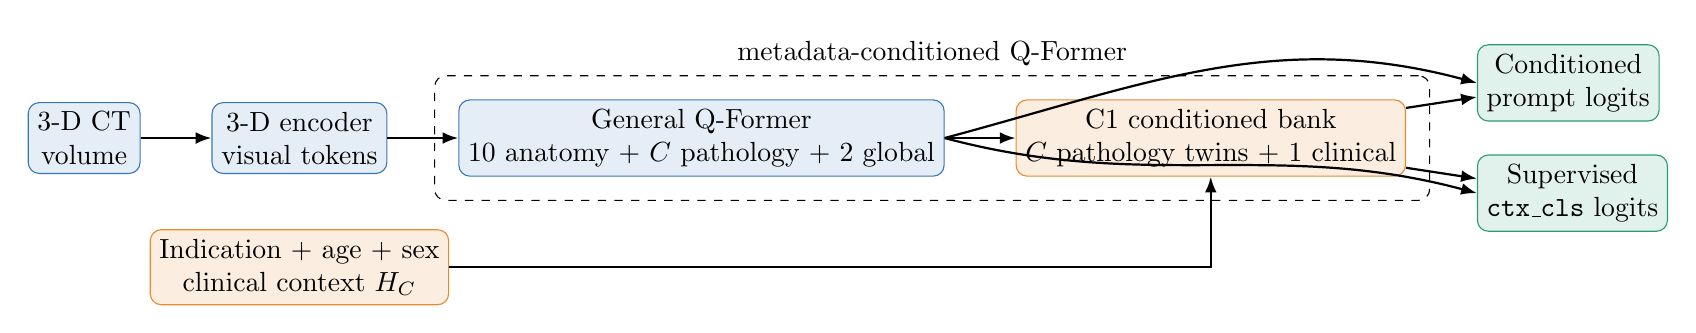
\begin{tikzpicture}[
  node distance=7mm and 9mm,
  block/.style={draw,rounded corners,minimum height=9mm,align=center,fill=lightgray},
  general/.style={block,fill=ctblue!13,draw=ctblue},
  context/.style={block,fill=ctxorange!15,draw=ctxorange},
  output/.style={block,fill=ctxgreen!14,draw=ctxgreen},
  arrow/.style={-{Latex[length=2mm]},thick}
]
\node[general] (ct) {3-D CT\\volume};
\node[general,right=of ct] (enc) {3-D encoder\\visual tokens};
\node[general,right=of enc] (qgen) {General Q-Former\\10 anatomy + $C$ pathology + 2 global};
\node[context,below=of enc] (meta) {Indication + age + sex\\clinical context $H_C$};
\node[context,right=of qgen] (c1) {C1 conditioned bank\\$C$ pathology twins + 1 clinical};
\node[output,right=of c1,yshift=7mm] (prompt) {Conditioned\\prompt logits};
\node[output,right=of c1,yshift=-7mm] (cls) {Supervised\\\texttt{ctx\_cls} logits};
\draw[arrow] (ct)--(enc);
\draw[arrow] (enc)--(qgen);
\draw[arrow] (meta)-|(c1);
\draw[arrow] (qgen)--(c1);
\draw[arrow] (c1)--(prompt);
\draw[arrow] (qgen.east) to[out=15,in=165] (prompt.west);
\draw[arrow] (c1)--(cls);
\draw[arrow] (qgen.east) to[out=-15,in=165] (cls.west);
\node[draw,dashed,rounded corners,fit=(qgen)(c1),inner sep=3mm,label=above:{metadata-conditioned Q-Former}] {};
\end{tikzpicture}
\caption{Architecture overview. The metadata-independent general bank is
retained, while pathology-specific conditioned twins attend to clinical
context through C1 cross-attention and FiLM. Prompt inference is the primary
novelty readout. \texttt{ctx\_cls} is a separate supervised auxiliary head.}
\label{fig:architecture}
\end{figure*}

\section{Experimental Design}
\subsection{Cohorts and splits}
\Cref{tab:cohorts} summarizes the controlled evaluation cohorts. The
historical age-$\geq5$ pediatric task excludes examinations below age five and removes four
adult-specific targets from both training and evaluation. The removed targets
are arterial wall calcification, coronary wall calcification, hiatal hernia,
and emphysema.
The frozen paper campaign retains all BCH examinations with $0\leq$age$<18$
while using the same 23 pediatric-relevant targets.
No CT-RATE scans are mixed into pediatric adaptation minibatches. Adult
knowledge enters only through the ARC-CT initialization lineage.

\begin{table*}[t]
\centering
\caption{Datasets and matched experimental splits.}
\label{tab:cohorts}
\begin{tabular}{@{}lrrrrp{5.7cm}@{}}
\toprule
Task & Train & Development & Final validation & Classes & Provenance \\
\midrule
Historical pediatric CT-only & 5,948 & 1,509 & --- & 23 & BCH age $\geq5$; patient-disjoint train/validation; the 1,507 scored cases are a subset of model-selection validation \\
Historical pediatric Refined C1 & 5,948 & 1,509 & --- & 23 & Same cohort/split; seed-matched CT-only parent; base frozen, C1 trained \\
New pediatric $<18$ protocol & 4,320 & 748 & 1,273 & 23 & MRN-disjoint train/development/test; includes ages 0--5; frozen campaign launched September 11, 2026 \\
Adult CT-only & 42,544 & 4,589 & 3,002 & 18 & CT-RATE only; official validation split \\
Adult Refined C1 & 42,544 & 4,589 & 3,002 & 18 & Same cohort/split; indication, scalar age, and sex conditioning \\
\bottomrule
\end{tabular}
\end{table*}

\subsection{Evaluation}
The primary endpoint is macro AUROC across trained targets. We report three
independent seeds for matched CT-only and Refined-C1 experiments. Pediatric age
strata include only classes with at least 10 positives and 10 negatives.
Non-AUROC benchmark metrics follow the CT-CLIP/ARC-CT convention: per-class
ROC-vertex thresholds, positive-class precision, accuracy, and support-weighted
F1, averaged over classes. We preserve fixed-threshold analyses separately and
do not mix their metrics with this protocol.

Patient-specific context usage is tested without retraining by evaluating each
Refined-C1 checkpoint with (i) the correct indication, (ii) all indications
blanked, and (iii) indications shuffled across patients. This intervention
isolates semantic context use from extra model capacity.

\subsection{Split audit and frozen pediatric paper protocol}
An MRN-level audit found no patient overlap between the historical clean BCH
training and validation pools. It also found that the previously described
1,507-case ``final'' cohort was not an independent test set: all 1,507 scored
cases were contained in the 1,509-case Stage-2 model-selection validation
list. We therefore relabel those results as historical held-out validation and
do not describe them as sealed test performance.

For the frozen paper campaign, we retain every study with $0\leq$age$<18$,
including ages 0--5, and use the same genuine 23-target schema. The historical
training pool was divided by MRN into 4,320 training studies (2,108 patients)
and 748 development studies (373 patients). The historical patient-disjoint
validation pool contributes 1,273 test studies (611 patients). Patient overlap
is zero for every pair of splits. Because this source validation pool was
inspected during earlier exploratory work, we call this a frozen retrospective
test rather than claiming a never-observed prospective test.

\begin{table*}[t]
\centering
\caption{Live pediatric paper experiment ledger. A dash means that no result
is yet available. Queued jobs are not completed evidence.}
\label{tab:live-pediatric-ledger}
\begin{tabularx}{\textwidth}{@{}llXl@{}}
\toprule
Track & Scheduler ID & Deliverable & Status at September 12, 2026 \\
\midrule
Historical age-$\geq5$ completion & 23949615 & Missing C1/C2, metadata, anatomy, routing, alignment, mask, prompt, and training-recipe arms & Running/queued \\
Historical age-$\geq5$ evaluation & 23949616, 23949617 & Consistent prompt, per-class, and age-stratified outputs & Dependency queued/running \\
Historical age-$\geq5$ table render & 23951526 & Refresh every completed transferred-recipe arm in the imported \LaTeX{} table & Partial table generated; final refresh dependency queued \\
True-pediatric smoke tests & 23949882, 23949883 & Stage-1 plus full, cross-attention-only, FiLM-only, and naive-fusion startup checks & Completed successfully \\
True-pediatric Stage-1 & 23949884 & R(2+1)D-18 adaptation on the $<18$ train/development split & Completed; best development AUROC 0.7868 \\
True-pediatric architecture matrix & 24078222 & 35 controlled arms, including three full-model and three CT-only seeds & Recovered; current development bests are 0.8083/0.8099/0.8058 for full seeds and 0.7642/0.7600/0.7615 for CT-only seeds; C2-off/C1-off currently reach 0.7900/0.7534 and will resume from preserved checkpoints; these unequal-boundary values are not the final comparison \\
Preserved-checkpoint evaluation & 24078219--24078221 & Immediate test evaluation of the saved all-age, age-$\geq5$, and R3D checkpoints & Completed successfully; interim results reported below with patient-bootstrap intervals \\
Evening snapshot evaluation & 24079753, 24079755, 24079756; aggregation 24086573, 24086574 & Re-evaluate all checkpoint-bearing all-age, age-$\geq5$, and R3D arms at 20:00 without stopping continued training, then generate snapshot-specific core, subgroup, per-class, and age-factorial \LaTeX{} tables & Completed: all 15 evaluations and both aggregations exited 0; all-age Full versus CT-only test AUROC is 0.8268 versus 0.7687 ($\Delta=+0.0581$, patient-bootstrap 95\% CI [0.0482, 0.0685], $p<0.001$) \\
True-pediatric standard evaluation & 24078286 & Test AUROC, AUPRC, calibration, sensitivity at fixed specificity, MRN-bootstrap confidence intervals, per-class, and age-stratified outputs for all arms & After-any recovery dependency, so one failed arm cannot block the others \\
True/blank/shuffled indication & 24078287 & Three-seed indication intervention on the $<18$ test split & After-any recovery dependency \\
Extended-ablation evaluation & 24078286 & Prompt, calibration, and fixed-specificity metrics for the extended controlled arms & Included in the recovered evaluation array \\
Age 0--5 factorial & 24078223, 24078288, 24079675 & Matched $<18$ versus 5--$<18$ Stage-1, three-seed Full/CT-only Stage-2, identical 5--$<18$ test evaluation, and MRN-bootstrap comparison & Training continues; current full-seed development bests are 0.8120/0.8141/0.8220 and CT-only seed bests are 0.7923/0.7909/0.7888. The completed snapshot factorial finds that excluding ages 0--5 changes Full AUROC by $-0.0075$ (95\% CI [$-0.0136$, $-0.0008$]) but CT-only by $+0.0250$ ([0.0154, 0.0344]) \\
Backbone ablation & 24078224, 24078289 & U18 R3D-18 Stage-1 plus matched full-model Stage-2/evaluation against primary R(2+1)D-18 & Training continues; best development AUROC is 0.8012 and the completed snapshot test AUROC is 0.8144, versus 0.8173 for matched R(2+1)D seed 0 \\
Pathology-specific prompt readout & 24078222 task 40, 24078286 task 40 & Conditioned pathology-token class-logit training and matched test evaluation & Relaunched in the recovered matrix \\
Final result-table render & 24078300 & Regenerate every completed U18 core, extended, backbone, and class-logit result into the \LaTeX{} paper fragment & After-any dependency queued \\
No-CT metadata controls & 23949963 & Indication-only, demographics-only, and all-metadata linear controls, three seeds each & Completed \\
Radiologist review packet & 24078302 & Sixty blinded indication-sensitive, multimodal-gain, and difficult CT cases plus a private analysis key & Recovery dependency queued; human scoring remains pending \\
Pediatric baseline benchmark & 24077477, 24077840, 24078457/8, 24093223 & Full saved-checkpoint sweep (21 checkpoints), CT-CLIP and VocabFine latent evaluation with a four-template prompt sweep, BiomedCLIP zero-shot plus linear probe, and Merlin linear probe; isolated under \texttt{PEDS\_BENCH} & Completed cleanly; ten measured rows in Table~\ref{tab:pedsbench}, each re-derived from its own saved predictions and verified against the labels file \\
\bottomrule
\end{tabularx}
\end{table*}

The registered 35-arm component matrix changes one factor at a time around the full
recipe: CT-only, C1 off, C2 off, cross-attention only, FiLM only, indication
only, demographics only, no metadata, naive pooled-metadata fusion, anatomy
queries off, routing off, regional alignment off, fully mask-free operation,
scalar versus banded age, indication dropout 0/0.1/0.3/0.4, augmentation off,
counterfactual loss, Qwen versus keyword region text, and the auxiliary
\texttt{ctx\_cls} head. It additionally tests L2 normalization, standard
versus null negative prompts, indication-loss weights 1/2/4, one/two/six global
queries, counterfactual weights 0/0.05/0.15, and general-versus-conditioned
checkpoint selection. Numerical cells will be populated only from completed
artifacts matched to their checkpoint, split, and readout.

\section{Results}
\IfFileExists{generated/peds23_u18_results.tex}{%
  \input{generated/peds23_u18_results.tex}%
}{%
  \subsection{Frozen true-pediatric ($<18$) results}
  Results are pending for the registered jobs in
  Table~\ref{tab:live-pediatric-ledger}. No numerical placeholders are treated
  as evidence.
}
\IfFileExists{generated/peds23_age_factorial.tex}{%
  \input{generated/peds23_age_factorial.tex}%
}{%
  The registered all-age-versus-age-$\geq5$ training factorial is pending.
}
\IfFileExists{generated/peds23_ge5_ablation.tex}{%
  % Auto-generated historical pediatric ablation table.
\subsection{Completed historical age-$\geq5$ current-recipe ablations}
\begin{table*}[t]
\centering
\caption{Completed current-recipe age-$\geq5$ 23-target ablations on the same historical validation split. Global denotes the conditioned/fused prompt readout; arms without a completed evaluation are omitted.}
\label{tab:peds-ge5-complete}
\begin{tabular}{@{}lrrrrr@{}}
\toprule
Arm & Global AUC & General AUC & Global F1 & Global accuracy & Global precision \\
\midrule
Full model, three-seed mean & 0.8387 & 0.8143 & 0.3644 & 0.8675 & 0.5082 \\
CT-only, three-seed mean & 0.8050 & 0.8050 & 0.3303 & 0.8729 & 0.5174 \\
\midrule
Full current model, seed 0 & 0.8370 & 0.8076 & 0.3134 & 0.8695 & 0.5334 \\
Full current model, seed 1 & 0.8393 & 0.8167 & 0.3400 & 0.8745 & 0.4924 \\
Full current model, seed 2 & 0.8399 & 0.8185 & 0.4397 & 0.8586 & 0.4987 \\
CT-only, seed 0 & 0.8177 & 0.8177 & 0.3738 & 0.8776 & 0.5820 \\
CT-only, seed 1 & 0.8159 & 0.8159 & 0.3514 & 0.8792 & 0.5517 \\
CT-only, seed 2 & 0.7813 & 0.7813 & 0.2657 & 0.8617 & 0.4185 \\
Indication dropout 0.4 & 0.8216 & 0.7882 & 0.3314 & 0.8512 & 0.4987 \\
C1 off & 0.8103 & 0.7893 & 0.2896 & 0.8016 & 0.3982 \\
Indication conditioning only & 0.8204 & 0.7883 & 0.3591 & 0.8152 & 0.3997 \\
Demographic conditioning only & 0.8085 & 0.7890 & 0.3874 & 0.8298 & 0.4060 \\
Standard negative prompts & 0.8201 & 0.7767 & 0.3348 & 0.8257 & 0.4523 \\
Auxiliary ctx\_cls & 0.8243 & 0.7880 & 0.3781 & 0.8391 & 0.4762 \\
Indication-loss weight 1 & 0.8200 & 0.7862 & 0.3520 & 0.8173 & 0.4350 \\
Indication-loss weight 4 & 0.8229 & 0.7893 & 0.3634 & 0.8359 & 0.4199 \\
Qwen region text & 0.8206 & 0.7877 & 0.4036 & 0.7958 & 0.3817 \\
One global query & 0.8221 & 0.7879 & 0.3274 & 0.8478 & 0.3971 \\
Six global queries & 0.8238 & 0.7940 & 0.3294 & 0.8044 & 0.4276 \\
Augmentation off & 0.8223 & 0.7795 & 0.3587 & 0.8039 & 0.3523 \\
\bottomrule
\end{tabular}
\end{table*}
\begin{table}[t]
\centering
\caption{Available current-recipe indication interventions on the age-$\geq5$ cohort. Only completed evaluations are shown.}
\label{tab:peds-ge5-intervention-final}
\begin{tabular}{@{}llr@{}}
\toprule
Seed & Indication & AUROC \\
\midrule
0 & Correct & 0.8370 \\
0 & Blank & 0.8180 \\
1 & Correct & 0.8393 \\
1 & Blank & 0.8204 \\
1 & Shuffled & 0.8107 \\
2 & Correct & 0.8399 \\
\bottomrule
\end{tabular}
\end{table}
%
}{%
  The complete historical age-$\geq5$ ablation render is pending.
}
\IfFileExists{generated/peds23_recovery_interim.tex}{%
  \subsection{Interim recovery results from preserved checkpoints}
The September 11 training wave was interrupted by a storage-quota error after
its first one or two validation boundaries.  Table~\ref{tab:peds-recovery}
reports frozen-test point estimates from the atomically saved checkpoints while
training resumes.  These values are useful early evidence, but they are not
substitutes for the preregistered completed-training comparison and confidence
intervals.  In particular, the age-$\geq5$ CT-only seed 2 checkpoint was not
written before the interruption.

\begin{table*}[t]
\centering
\caption{Interim 23-label pediatric frozen-test macro AUROC from preserved
checkpoints.  Full denotes the metadata-conditioned prompt branch; general is
the metadata-independent branch from the same full-model checkpoint.}
\label{tab:peds-recovery}
\begin{tabular}{@{}llrrrrl@{}}
\toprule
Cohort / architecture & Readout & Seed 0 & Seed 1 & Seed 2 & Mean & Qualification \\
\midrule
All age $<18$, R(2+1)D-18 & Full conditioned & 0.8210 & 0.8086 & 0.7994 & 0.8097 & updates 500--1000 \\
All age $<18$, R(2+1)D-18 & General branch & 0.7903 & 0.7726 & 0.7701 & 0.7777 & same checkpoints \\
All age $<18$, R(2+1)D-18 & Within-checkpoint $\Delta$ & +0.0307 & +0.0360 & +0.0293 & \best{+0.0320} & conditioned--general \\
\midrule
Age $\geq5$, R(2+1)D-18 & Full conditioned & 0.8295 & 0.8165 & 0.8121 & 0.8194 & updates 500--1000 \\
Age $\geq5$, R(2+1)D-18 & CT-only & 0.7873 & 0.7693 & --- & 0.7783 & two seeds available \\
Age $\geq5$, R(2+1)D-18 & Matched $\Delta$ & +0.0422 & +0.0472 & --- & \best{+0.0447} & paired two-seed mean \\
\midrule
All age $<18$, R3D-18 & Full conditioned & 0.8044 & --- & --- & 0.8044 & update 1000 \\
\bottomrule
\end{tabular}
\end{table*}

Patient-level 1,000-replicate bootstrap intervals for the all-age conditioned
AUROC are [0.8070, 0.8333], [0.7933, 0.8229], and [0.7838, 0.8133] for seeds
0--2.  The corresponding age-$\geq5$ intervals are [0.8149, 0.8420],
[0.8013, 0.8310], and [0.7958, 0.8271].  For the two available age-$\geq5$
CT-only controls they are [0.7691, 0.8041] and [0.7512, 0.7860].  Mean AUPRC
is 0.4380 for the all-age conditioned checkpoints, 0.4442 for the age-$\geq5$
conditioned checkpoints, and 0.3760 for the two age-$\geq5$ CT-only controls.
%
}{}
\IfFileExists{generated/peds23_u18_snapshot.tex}{%
  % Auto-generated from audited prediction artifacts; do not edit by hand.
\subsection{20:00 true-pediatric checkpoint snapshot}
\begin{table}[t]
\centering
\caption{Interim 20:00 checkpoint snapshot on the MRN-disjoint $<18$ test split; training continued after evaluation.}
\label{tab:u18-primary-snapshot}
\begin{tabular}{@{}lrrr@{}}
\toprule
Seed & CT-only AUROC & Full AUROC & $\Delta$ \\
\midrule
0 & 0.7719 & 0.8173 & +0.0454 \\
1 & 0.7687 & 0.8313 & +0.0625 \\
2 & 0.7654 & 0.8317 & +0.0662 \\
\midrule
Mean & 0.7687 & 0.8268 & +0.0581 \\
\bottomrule
\end{tabular}
\parbox{\columnwidth}{\footnotesize Patient-bootstrap 95\% CI for the mean paired AUROC difference: [0.0482, 0.0685]; two-sided paired bootstrap $p<0.001$.}
\end{table}
\begin{table*}[t]
\centering
\caption{Audited completed $<18$ checkpoint-snapshot and follow-up ablations. Arms without a completed frozen-test evaluation are omitted.}
\label{tab:u18-ablation-snapshot}
\begin{tabular}{@{}lrrlll@{}}
\toprule
Arm & AUROC & AUPRC & Brier & ECE & Sens.@95\% spec. \\
\midrule
Full model, seed 0 & 0.8173 & 0.4619 & 0.1155 & 0.1093 & 0.4307 \\
Full model, seed 1 & 0.8313 & 0.4547 & 0.1430 & 0.1546 & 0.4316 \\
Full model, seed 2 & 0.8317 & 0.4681 & 0.1069 & 0.0941 & 0.4504 \\
CT-only, seed 0 & 0.7719 & 0.3547 & 0.1012 & 0.0794 & 0.3321 \\
CT-only, seed 1 & 0.7687 & 0.3681 & 0.0959 & 0.0637 & 0.3303 \\
CT-only, seed 2 & 0.7654 & 0.3547 & 0.1025 & 0.0802 & 0.3263 \\
C2 off & 0.8126 & 0.4191 & 0.1119 & 0.1059 & 0.3842 \\
C1 off & 0.7629 & 0.3669 & 0.1292 & 0.1137 & 0.3534 \\
R3D-18 backbone, full model, seed 0 & 0.8144 & 0.4549 & 0.1010 & 0.0879 & 0.4227 \\
Asymmetric loss (ASL), seed 0 & 0.8055 & 0.4493 & 0.1016 & 0.0991 & 0.4017 \\
BCE + BNM ($\lambda=0.001$), seed 0 & 0.8305 & 0.4715 & 0.0989 & 0.0880 & 0.4430 \\
BCE + BNM ($\lambda=0.003$), seed 0 & 0.8301 & 0.4693 & 0.1000 & 0.0860 & 0.4370 \\
BCE + BNM ($\lambda=0.010$), seed 0 & 0.8298 & 0.4676 & 0.0955 & 0.0813 & 0.4292 \\
ASL + BNM ($\lambda=0.001$), seed 0 & 0.8190 & 0.4558 & 0.1882 & 0.2591 & 0.4118 \\
ASL + BNM ($\lambda=0.003$), seed 0 & 0.8172 & 0.4528 & 0.1614 & 0.2271 & 0.3998 \\
ASL + BNM ($\lambda=0.010$), seed 0 & 0.8158 & 0.4462 & 0.2103 & 0.2832 & 0.4110 \\
\bottomrule
\end{tabular}
\end{table*}
\begin{table}[t]
\centering
\caption{Age and sex subgroup consistency on the $<18$ test split.}
\label{tab:u18-subgroups-snapshot}
\begin{tabular}{@{}llrr@{}}
\toprule
Subgroup & Model & $N$ & AUROC \\
\midrule
age\_0\_2 & ct\_only & 105 & 0.7185 \\
age\_0\_2 & full & 105 & 0.7609 \\
age\_2\_5 & ct\_only & 147 & 0.7509 \\
age\_2\_5 & full & 147 & 0.8051 \\
age\_5\_10 & ct\_only & 252 & 0.7200 \\
age\_5\_10 & full & 252 & 0.7807 \\
age\_10\_15 & ct\_only & 435 & 0.7825 \\
age\_10\_15 & full & 435 & 0.8478 \\
age\_15\_18 & ct\_only & 334 & 0.7427 \\
age\_15\_18 & full & 334 & 0.8066 \\
sex\_F & ct\_only & 681 & 0.7715 \\
sex\_F & full & 681 & 0.8315 \\
sex\_M & ct\_only & 592 & 0.7603 \\
sex\_M & full & 592 & 0.8179 \\
exam\_year\_2011\_2018 & ct\_only & 615 & 0.7809 \\
exam\_year\_2011\_2018 & full & 615 & 0.8427 \\
exam\_year\_2019\_2026 & ct\_only & 658 & 0.7587 \\
exam\_year\_2019\_2026 & full & 658 & 0.8090 \\
acquisition\_site\_rank\_1 & ct\_only & 413 & 0.7516 \\
acquisition\_site\_rank\_1 & full & 413 & 0.8057 \\
acquisition\_site\_rank\_2 & ct\_only & 293 & 0.7089 \\
acquisition\_site\_rank\_2 & full & 293 & 0.7816 \\
acquisition\_site\_rank\_3 & ct\_only & 135 & 0.7164 \\
acquisition\_site\_rank\_3 & full & 135 & 0.7792 \\
acquisition\_site\_rank\_4 & ct\_only & 116 & 0.7078 \\
acquisition\_site\_rank\_4 & full & 116 & 0.7649 \\
\bottomrule
\end{tabular}
\end{table}
\begin{table}[t]
\centering
\caption{Performance stratified by explicit target terminology in the indication.}
\label{tab:u18-mention-strata-snapshot}
\begin{tabular}{@{}llrr@{}}
\toprule
Terminology & Model & AUROC & AUPRC \\
\midrule
explicit\_term\_present & ct\_only & 0.6694 & 0.6771 \\
explicit\_term\_present & full & 0.7153 & 0.7339 \\
explicit\_term\_absent & ct\_only & 0.7692 & 0.3494 \\
explicit\_term\_absent & full & 0.8249 & 0.4486 \\
\bottomrule
\end{tabular}
\end{table}
\begin{table*}[t]
\centering
\caption{Complete three-seed per-class results on the frozen $<18$ test split.}
\label{tab:u18-per-class-snapshot}
\begin{tabular}{@{}lrrrrrrr@{}}
\toprule
Class & Pos. & CT AUC & Full AUC & $\Delta$ AUC & CT AUPRC & Full AUPRC & $\Delta$ AUPRC \\
\midrule
Medical material & 535 & 0.8941 & 0.9225 & +0.0283 & 0.8649 & 0.9061 & +0.0412 \\
Cardiomegaly & 29 & 0.9185 & 0.9609 & +0.0424 & 0.2857 & 0.4413 & +0.1556 \\
Pericardial effusion & 44 & 0.8471 & 0.9024 & +0.0553 & 0.1890 & 0.2753 & +0.0862 \\
Lymphadenopathy & 96 & 0.7745 & 0.7602 & -0.0142 & 0.2616 & 0.2732 & +0.0115 \\
Atelectasis & 447 & 0.7270 & 0.7465 & +0.0195 & 0.6210 & 0.6560 & +0.0350 \\
Lung nodule & 631 & 0.6579 & 0.6891 & +0.0312 & 0.6223 & 0.6656 & +0.0433 \\
Lung opacity & 426 & 0.7438 & 0.7741 & +0.0303 & 0.6080 & 0.6536 & +0.0456 \\
Pulmonary fibrotic sequela & 235 & 0.6614 & 0.7682 & +0.1068 & 0.3138 & 0.4332 & +0.1194 \\
Pleural effusion & 48 & 0.9559 & 0.9640 & +0.0081 & 0.5193 & 0.6318 & +0.1125 \\
Mosaic attenuation pattern & 185 & 0.7351 & 0.8253 & +0.0901 & 0.3540 & 0.4362 & +0.0823 \\
Peribronchial thickening & 168 & 0.7960 & 0.8352 & +0.0392 & 0.4607 & 0.5047 & +0.0439 \\
Consolidation & 76 & 0.8632 & 0.8922 & +0.0290 & 0.4035 & 0.4380 & +0.0346 \\
Bronchiectasis & 103 & 0.9004 & 0.9337 & +0.0334 & 0.5713 & 0.7101 & +0.1388 \\
Interlobular septal thickening & 76 & 0.8444 & 0.8818 & +0.0374 & 0.3224 & 0.4314 & +0.1090 \\
Post-surgical or post-treatment change & 392 & 0.6754 & 0.8150 & +0.1396 & 0.4952 & 0.6828 & +0.1876 \\
Pulmonary metastases & 76 & 0.6155 & 0.8170 & +0.2014 & 0.1397 & 0.2708 & +0.1311 \\
Tree-in-bud & 90 & 0.7893 & 0.8602 & +0.0709 & 0.3177 & 0.4501 & +0.1324 \\
Pulmonary cyst & 50 & 0.6645 & 0.7251 & +0.0606 & 0.0690 & 0.1199 & +0.0509 \\
Mass or neoplasm & 33 & 0.7224 & 0.8218 & +0.0994 & 0.1285 & 0.2556 & +0.1271 \\
Mucus plugging & 44 & 0.7891 & 0.8378 & +0.0487 & 0.1760 & 0.2986 & +0.1226 \\
Pleural thickening or nodule & 146 & 0.6757 & 0.6950 & +0.0193 & 0.2283 & 0.2630 & +0.0347 \\
Bone lesion or fracture & 179 & 0.5925 & 0.6699 & +0.0774 & 0.2016 & 0.3056 & +0.1040 \\
Pneumothorax & 25 & 0.8363 & 0.9176 & +0.0814 & 0.1072 & 0.5136 & +0.4065 \\
\bottomrule
\end{tabular}
\end{table*}
%
}{}
\IfFileExists{generated/peds23_age_factorial_snapshot.tex}{%
  % Auto-generated age-factorial result.
\subsection{20:00 checkpoint snapshot: does excluding ages 0--5 help?}
\begin{table}[t]
\centering
\caption{Interim 20:00 age-training checkpoint snapshot evaluated on the identical 5--$<18$ MRN-disjoint test subset.}
\label{tab:peds-age-factorial-snapshot}
\begin{tabular}{@{}llrr@{}}
\toprule
Model & Training ages & AUROC & AUPRC \\
\midrule
CT-only & 0--$<18$ & 0.7656 & 0.3573 \\
CT-only & 5--$<18$ & 0.7907 & 0.4110 \\
Full & 0--$<18$ & 0.8287 & 0.4689 \\
Full & 5--$<18$ & 0.8212 & 0.4503 \\
\bottomrule
\end{tabular}
\parbox{\columnwidth}{\footnotesize CT-only: excluding ages 0--5 changes AUROC by +0.0250 (patient-bootstrap 95\% CI [0.0154, 0.0344]).}
\parbox{\columnwidth}{\footnotesize Full: excluding ages 0--5 changes AUROC by -0.0075 (patient-bootstrap 95\% CI [-0.0136, -0.0008]).}
\end{table}
%
}{}
\paragraph{Interpretation of the 20:00 checkpoint snapshot.}
Across three seeds, metadata-conditioned prompt inference improves frozen-test
macro AUROC from 0.7687 to 0.8268 ($\Delta=+0.0581$, patient-bootstrap 95\%
CI [0.0482, 0.0685], $p<0.001$) and macro AUPRC from 0.3592 to 0.4616
($\Delta=+0.1024$, 95\% CI [0.0830, 0.1198]). The AUROC gain is positive
in every prespecified age bin and in both sex strata. In the single-seed
component snapshot, removing C1 lowers AUROC from 0.8173 to 0.7629, whereas
removing C2 yields 0.8126. This interim evidence identifies token-level C1
conditioning as the larger contributor, while the converged matrix remains
necessary for a final component claim. Training only on ages 5--$<18$ does
not improve the Full model on the identical 5--$<18$ test cases
($\Delta=-0.0075$, 95\% CI [$-0.0136$, $-0.0008$]), arguing against removal
of younger children from the primary pediatric cohort. Finally, replacing
R(2+1)D-18 with R3D-18 changes the matched seed-0 AUROC from 0.8173 to 0.8144,
indicating little backbone sensitivity at this checkpoint.
\subsection{Matched pediatric and adult performance}

\begin{table}[t]
\centering
\caption{Historical matched prompt-inference validation results (macro AUROC,
mean $\pm$ SD over three seeds). These are not independent test estimates.}
\label{tab:main}
\begin{tabular}{@{}lccc@{}}
\toprule
Task & CT-only & Refined C1 & $\Delta$ \\
\midrule
Pediatric, 23 labels & 0.7933$\pm$.0017 & \best{0.8396$\pm$.0015} & \best{+0.0463} \\
CT-RATE, 18 labels (final checkpoint) & 0.8733 & \best{0.8781} & \best{+0.0048} \\
\bottomrule
\end{tabular}
\end{table}

\begin{figure}[t]
\centering
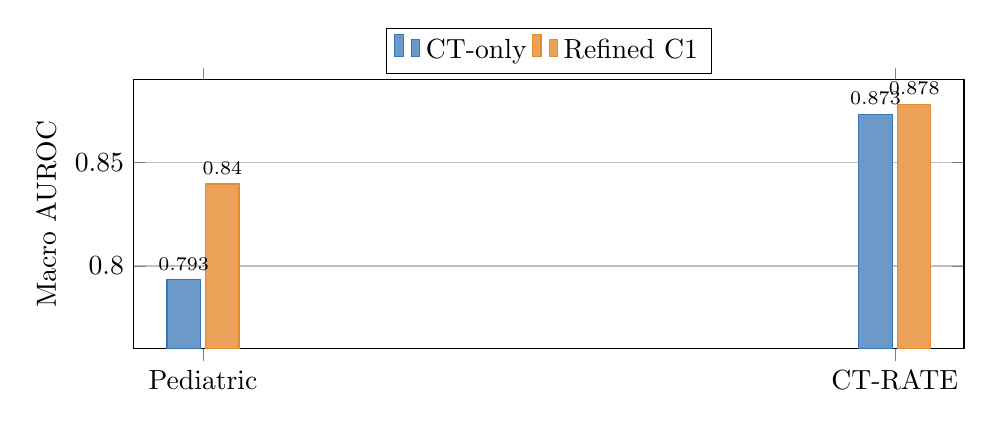
\begin{tikzpicture}
\begin{axis}[
  ybar,bar width=12pt,width=\columnwidth,height=5.0cm,
  ymin=0.76,ymax=0.89,ymajorgrids=true,
  symbolic x coords={Pediatric,CT-RATE},xtick=data,
  ylabel={Macro AUROC},legend style={at={(0.5,1.02)},anchor=south,legend columns=2},
  nodes near coords,nodes near coords style={font=\scriptsize,/pgf/number format/fixed,/pgf/number format/precision=3}
]
\addplot[fill=ctblue!75,draw=ctblue] coordinates {(Pediatric,0.7933) (CT-RATE,0.8733)};
\addplot[fill=ctxorange!80,draw=ctxorange] coordinates {(Pediatric,0.8396) (CT-RATE,0.8781)};
\legend{CT-only,Refined C1}
\end{axis}
\end{tikzpicture}
\caption{Refined C1 improves both matched tasks, with a substantially larger
gain in the pediatric cohort.}
\label{fig:mainbars}
\end{figure}

All three pediatric C1 seeds exceed 0.83 and improve over their matched
controls (Table~\ref{tab:pedsseeds}). The gain is also positive in every
reported age stratum (Table~\ref{tab:age}).

\begin{table}[t]
\centering
\caption{Pediatric seed and indication intervention results.}
\label{tab:pedsseeds}
\resizebox{\columnwidth}{!}{%
\begin{tabular}{@{}lrrrr@{}}
\toprule
Arm & Seed 0 & Seed 1 & Seed 2 & Mean \\
\midrule
CT-only & 0.7934 & 0.7950 & 0.7916 & 0.7933 \\
C1, correct & \best{0.8386} & \best{0.8414} & \best{0.8389} & \best{0.8396} \\
C1, blank & 0.8111 & 0.8091 & 0.8074 & 0.8092 \\
C1, shuffled & 0.7980 & 0.7967 & 0.7934 & 0.7960 \\
\bottomrule
\end{tabular}}
\end{table}

\subsection{Does the model use the correct indication?}
In pediatrics, correct indications outperform blank and shuffled indications by
3.04 and 4.36 AUROC points, respectively. Shuffling removes almost the entire
gain over CT-only. In adults, the corresponding differences are only 0.20 and
0.31 points (Fig.~\ref{fig:intervention}). Thus, rich pediatric indications
provide patient-specific diagnostic information, whereas much of the adult
gain reflects the learned class-specific adaptation rather than indication
semantics alone.

\begin{figure}[t]
\centering
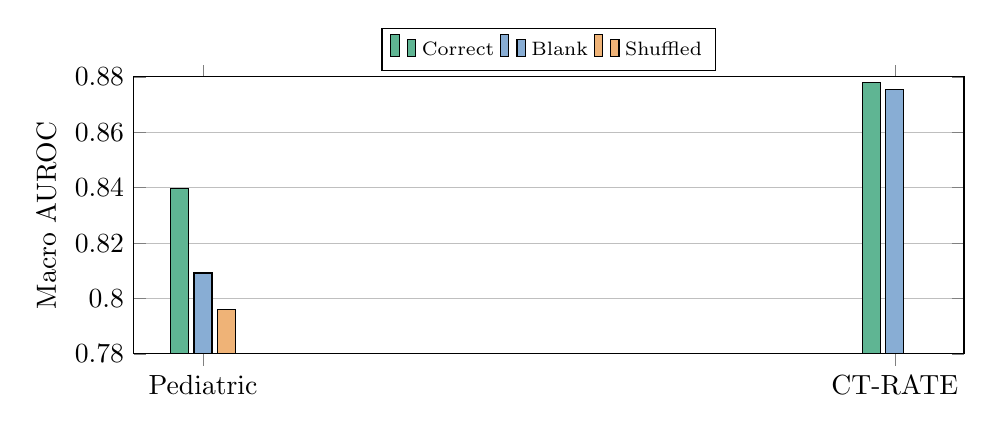
\begin{tikzpicture}
\begin{axis}[
  ybar,bar width=6.5pt,width=\columnwidth,height=5.1cm,
  ymin=0.78,ymax=0.88,ymajorgrids=true,
  symbolic x coords={Pediatric,CT-RATE},xtick=data,
  ylabel={Macro AUROC},
  legend style={at={(0.5,1.02)},anchor=south,legend columns=3,font=\scriptsize}
]
\addplot[fill=ctxgreen!75] coordinates {(Pediatric,0.8396) (CT-RATE,0.8781)};
\addplot[fill=ctblue!60] coordinates {(Pediatric,0.8092) (CT-RATE,0.8754)};
\addplot[fill=ctxorange!65] coordinates {(Pediatric,0.7960)};
\legend{Correct,Blank,Shuffled}
\end{axis}
\end{tikzpicture}
\caption{Inference-time indication intervention on the same trained
checkpoints. Pediatric predictions depend strongly on the correct indication.
The adult dependence is much smaller. The adult shuffled arm is not yet
available on the final checkpoint, so no adult bar is drawn for it.}
\label{fig:intervention}
\end{figure}

\begin{table}[t]
\centering
\caption{Pediatric performance by age. Only eligible classes enter each
stratum's macro AUROC.}
\label{tab:age}
\begin{tabular}{@{}lrrrr@{}}
\toprule
Age & $N$ & Classes & CT-only & C1 ($\Delta$) \\
\midrule
5--10 & 252 & 15 & 0.7451 & \best{0.7904} (+.0452) \\
10--18 & 768 & 23 & 0.7995 & \best{0.8440} (+.0445) \\
18--25 & 402 & 20 & 0.7729 & \best{0.8190} (+.0461) \\
25+ & 85 & 15 & 0.7615 & \best{0.8050} (+.0435) \\
All $<18$ & 1,020 & 23 & 0.7979 & \best{0.8412} (+.0433) \\
All $\geq18$ & 487 & 23 & 0.7841 & \best{0.8325} (+.0483) \\
\midrule
Pooled & 1,507 & 23 & 0.7933 & \best{0.8396} (+.0463) \\
\bottomrule
\end{tabular}
\end{table}

\subsection{How predictive is metadata without the CT?}
To measure clinical-prior strength and potential indication leakage directly,
we freeze the same CXR-BERT indication encoder and fit only a LayerNorm and
linear 23-label head, with no CT input. Table~\ref{tab:metadata-only} reports
three-seed results on the new $<18$ test split. Indication alone is strongly
predictive, whereas age and sex alone are near chance. Adding demographics to
the indication gives only a small additional gain. Consequently, the full
multimodal model must outperform both the matched CT-only model and the
metadata-only control. Beating CT-only alone is insufficient evidence of
visual--clinical fusion.

\begin{table}[t]
\centering
\caption{No-CT controls on the frozen $<18$ test split ($N=1,273$). AUROC is
mean $\pm$ SD over three linear-head seeds. AUPRC is the three-seed mean.}
\label{tab:metadata-only}
\begin{tabular}{@{}lcc@{}}
\toprule
Input (no CT) & Macro AUROC & Macro AUPRC \\
\midrule
Age + sex & $0.5064\pm0.0065$ & 0.1578 \\
Indication & $0.7860\pm0.0003$ & 0.3792 \\
Indication + age + sex & $0.7867\pm0.0010$ & 0.3801 \\
\bottomrule
\end{tabular}
\end{table}

A conservative case-insensitive terminology audit found that at least one
positive target was explicitly named in the indication for 1,064/4,320
(24.6\%) training studies, 169/748 (22.6\%) development studies, and 330/1,273
(25.9\%) test studies. This heuristic does not distinguish a suspected disease
from a confirmed diagnosis and therefore is not itself proof of leakage. We
will report model performance separately for explicitly mentioned and
non-mentioned positive targets, alongside true/blank/shuffled indication
interventions, to determine whether gains extend beyond direct lexical cues.

\subsection{Pediatric benchmark context}
Because no published pediatric benchmark uses this exact BCH cohort and
23-label task, we evaluate comparison methods locally (Table~\ref{tab:pedsbench}).
These rows are not published pediatric results. CT-CLIP, CT-CLIP VocabFine,
H-LIP, and BiomedCLIP are evaluated from released weights without pediatric
training. The MPS-CT and GreenRFM rows are local pediatric
reproductions/adaptations, and the BiomedCLIP and Merlin probe rows fit a
linear head on frozen features of the pediatric training split. For methods
with multiple saved checkpoints, selection is by validation macro AUROC under
the same best-of-$N$ principle used for our models: MPS-CT peaks at update
3,000 (0.6961), while the GreenRFM supervised adaptation peaks at epoch 9/10
(0.7477). We note that this selection rule changed both baselines by at most
0.001 relative to their final checkpoints, so the earlier last-checkpoint
figures were not materially understated.

Several qualifications prevent this table from being read as a like-for-like
architecture ranking. The prompt methods do not receive identical inputs: our
method additionally receives patient metadata. The GreenRFM shared-head and
the two probe rows are supervised readouts. Merlin is an abdominal model and
BiomedCLIP is a 2-D model applied slice-wise, so both are reference points
rather than matched volumetric CT baselines. The clean causal comparison
remains Refined C1 versus its matched CT-only control.

One comparison nevertheless deserves comment. A linear probe on frozen
BiomedCLIP features (0.7643) exceeds every purpose-built volumetric CT
foundation model we could evaluate on this cohort, including the GreenRFM
supervised adaptation (0.7477) and MPS-CT (0.6961), despite BiomedCLIP having
no three-dimensional context whatsoever. Its per-class profile makes the
mechanism explicit: it is competitive on findings legible in a single axial
section and at chance on lung nodules. We read this as evidence that a
substantial part of current volumetric pretraining benefit on pediatric CT is
recoverable from a general-purpose 2-D biomedical encoder, and as a reason to
report pediatric baselines by measurement rather than by inheriting adult
CT-RATE rankings.

\begin{table*}[t]
\centering
\begin{threeparttable}
\caption{Pediatric benchmark evaluation on the same 1,507 studies (648
patients) and 23 labels. All values are locally measured macro AUROC, not
published pediatric results. Rows are grouped by whether the method was
adapted to the pediatric cohort, because a pediatric-adapted model and an
untrained transfer answer different questions and should not be ranked in a
single list. Intervals are 1,000-sample bootstrap resampling \emph{patients},
not studies. The cohort averages 2.33 studies per child, and resampling
studies understates the interval by roughly 35\%.}
\label{tab:pedsbench}
\small
\begin{tabular}{@{}llccp{4.6cm}@{}}
\toprule
Method & Readout & AUROC & 95\% CI & Qualification \\
\midrule
\multicolumn{5}{@{}l}{\emph{Adapted to the pediatric cohort}}\\
\ours{} Refined C1 & conditioned prompt & \best{0.8396}\tnote{a} & --- & three-seed historical campaign \\
Our CT-only & prompt & 0.7933\tnote{a} & --- & matched three-seed control \\
BiomedCLIP, linear probe & supervised probe & 0.7643 & 0.7473--0.7803 & 2-D encoder, 32 axial slices, mean-pooled\tnote{b} \\
GreenRFM, local adaptation & supervised head & 0.7477 & 0.7310--0.7637 & best of 10 saved checkpoints (epoch 9) \\
Merlin, linear probe & supervised probe & 0.7144 & 0.6951--0.7313 & abdominal/pelvic CT model\tnote{c} \\
MPS-CT, local reproduction & zero-shot prompt & 0.6961 & 0.6840--0.7089 & best of 12 saved checkpoints (update 3,000) \\
GreenRFM, local reproduction & zero-shot prompt & 0.6620 & --- & prompt readout is ill-posed for this model\tnote{d} \\
\addlinespace
\multicolumn{5}{@{}l}{\emph{Released adult weights, no pediatric training}}\\
BiomedCLIP & zero-shot prompt & 0.6938 & 0.6695--0.7108 & fixed prompt pair, no tuning\tnote{b} \\
H-LIP & zero-shot prompt & 0.6916 & 0.6763--0.7048 & released CT-RATE weights \\
CT-CLIP & zero-shot prompt & 0.5478 & 0.5277--0.5670 & best of the four templates in the released code\tnote{e} \\
CT-CLIP VocabFine & zero-shot prompt & 0.5339 & 0.5113--0.5572 & second released CT-CLIP variant\tnote{e} \\
\bottomrule
\end{tabular}
\begin{tablenotes}[flushleft]\footnotesize
\item[a] Historical Refined-C1 campaign (scalar age, 10\% indication dropout),
reported with three-seed standard deviations in Table~\ref{tab:main} rather
than a bootstrap interval. The remaining rows are single trained models scored
with the identical metric code on the identical split.
\item[b] BiomedCLIP is a 2-D biomedical vision--language model applied
slice-wise with no inter-slice context, so findings defined by
three-dimensional extent are invisible to it by construction: it reaches 0.503
(chance) on lung nodule against 0.935 on pleural effusion. It is included as a
deliberately non-CT-specific reference point, not as an architecture-matched
comparison. Its probe regularization was selected by patient-grouped
cross-validation on the pediatric training split alone.
\item[c] Merlin is an abdominal/pelvic CT foundation model, so this row is
out-of-domain on both body region and adult-to-pediatric transfer. Its
preprocessing also resamples to 3\,mm slices and discards thin-slice detail.
\item[d] GreenRFM's contrastive objective uses unnormalized dot products at
fixed temperature, so per-volume embedding norm enters the cross-volume
ranking. Its published adult result is the supervised head, which is the row
above. We report the prompt value only for completeness.
\item[e] Sweeping all four prompt templates shipped in the CT-CLIP repository
spans 0.528--0.548, so the low value is not a template artifact. A supervised
probe fitted on CT-CLIP's own image latents reaches only 0.609, indicating a
representational rather than a readout limitation on pediatric CT.
\end{tablenotes}
\end{threeparttable}
\end{table*}

\subsection{Pediatric report--CT retrieval}
On the same 1,507-study pediatric cohort we also measured report$\rightarrow$image
Recall@K and image$\rightarrow$image label-Jaccard@K for every reproducible
method, with no retrieval-specific fitting. The table is generated from the
audited prediction artifacts. The complete model, Refined C1 reading out
$\mathrm{norm}(z_{\mathrm{gen}}{+}z_{\mathrm{ind}})$, leads every prior method on
all ten columns. It reaches 9.5/15.5/39.9/51.7 on report$\rightarrow$image and
32.2/30.9/27.7 on clean image$\rightarrow$image Jaccard. The cross-model table
lists only the full model and its matched CT-only control.
\Cref{tab:pedsretrieval-readout} separates our readouts. There the
metadata-free $z_{\mathrm{gen}}$ (shared by CT-only and Refined C1, whose base
is frozen) retrieves the exact report best, at R@5/10/50/100 of
10.8/17.1/41.2/54.2, in the range of the published adult CT-RATE values, while
the conditioned $z_{\mathrm{ind}}$ retrieves the most label-similar studies
best (33.4 Jaccard at $K{=}5$): indication text sharpens what a study is a case
of and blurs which report was dictated for it. MPS-CT is the strongest prior
method (6.3/10.7/29.1/42.6), then H-LIP (3.6), BiomedCLIP (1.9) and Merlin
(1.0). Released CT-CLIP
and pediatric-adapted GreenRFM are at chance for report$\rightarrow$image,
GreenRFM because its unnormalized fixed-temperature contrastive space does not
support cosine retrieval, the same defect that voids its prompt readout. The
table reports image$\rightarrow$image both with the query excluded from its
gallery and in the CT-CLIP-script convention that prior tables (including
Table~4 of the ARC-CT paper) inherit, which includes the query and accumulates
across $K$. The two differ by roughly 20--40 points on identical latents.
Text context length is disclosed rather than equalised: at their published
lengths, Merlin's 1,024 tokens truncate 5 of the 1,507 reports and CT-CLIP's
and H-LIP's 512 truncate about 107, while the 128 that GreenRFM and MPS-CT
train with truncate 1,368 (91\%) against a 267-token median, bounding their
recall but not their image$\rightarrow$image scores.
\IfFileExists{generated/peds23_retrieval.tex}{%
  % Auto-generated by retr_make_table.py from PEDS_BENCH/retrieval/results; do not edit by hand.
\begin{table*}[t]\centering
\caption{Pediatric cross-modal retrieval on the historical cohort (1,507 studies, 648 patients), no retrieval-specific fitting. Report$\rightarrow$image is exact-match Recall@K over all 1,507 studies. Image$\rightarrow$image is mean label-set Jaccard of the top-$K$ retrieved studies (gallery = studies with $\geq$1 positive label): \emph{clean} excludes the query from its own gallery; \emph{Table-4 convention} reproduces the CT-CLIP evaluation script used by prior work, which includes the query and accumulates across $K$, and is shown only for comparability with published adult tables. Our arms are three-seed means; chance Recall@K is $K/N$.}
\label{tab:pedsretrieval}\small
\resizebox{\textwidth}{!}{%
\begin{tabular}{@{}lrrrrrrrrrr@{}}\toprule
 & \multicolumn{4}{c}{Report$\rightarrow$image R@K} & \multicolumn{3}{c}{Image$\rightarrow$image, clean} & \multicolumn{3}{c}{Image$\rightarrow$image, Table-4 conv.}\\
\cmidrule(lr){2-5}\cmidrule(lr){6-8}\cmidrule(lr){9-11}
Method & @5 & @10 & @50 & @100 & @5 & @10 & @50 & @5 & @10 & @50 \\ \midrule
\multicolumn{11}{@{}l}{\emph{Adapted to the pediatric cohort}}\\
\ours{} (full, metadata-conditioned)$^{\mathrm{m}}$ & 9.5$\pm$0.4 & 15.5$\pm$0.2 & 39.9$\pm$0.6 & 51.7$\pm$1.4 & \best{32.2$\pm$0.6} & \best{30.9$\pm$0.6} & \best{27.7$\pm$0.4} & \best{67.7} & \best{57.5} & \best{50.4} \\
\ours{} / CT-only control (metadata-free) & \best{10.8$\pm$0.6} & \best{17.1$\pm$0.1} & \best{41.2$\pm$0.4} & \best{54.2$\pm$1.2} & 31.7$\pm$0.2 & 30.4$\pm$0.3 & 27.5$\pm$0.1 & 67.4 & 57.2 & 50.1 \\
GreenRFM, local adaptation (epoch 9) & 0.3 & 1.1 & 5.4 & 9.4 & 27.8 & 26.2 & 23.4 & 66.0 & 54.9 & 47.4 \\
MPS-CT, local reproduction (update 3,000) & 6.3 & 10.7 & 29.1 & 42.6 & 30.9 & 28.4 & 24.2 & 67.3 & 56.5 & 48.8 \\
\multicolumn{11}{@{}l}{\emph{Released weights, no pediatric training}}\\
H-LIP & 3.6 & 5.8 & 14.9 & 22.4 & 23.7 & 22.6 & 20.8 & 64.2 & 52.7 & 45.0 \\
BiomedCLIP (2-D, slice-wise) & 1.9 & 3.3 & 11.8 & 17.4 & 25.3 & 23.8 & 21.0 & 64.9 & 53.5 & 45.8 \\
Merlin (abdominal) & 1.0 & 1.7 & 6.2 & 10.9 & 21.8 & 21.3 & 19.9 & 63.4 & 51.7 & 44.1 \\
CT-CLIP & 0.9 & 1.3 & 5.4 & 10.2 & 19.8 & 19.4 & 18.8 & 62.6 & 50.6 & 43.0 \\
CT-CLIP VocabFine & 0.3 & 0.9 & 3.7 & 6.7 & 20.8 & 20.0 & 19.1 & 62.9 & 51.0 & 43.4 \\
\midrule Chance ($K/N$) & 0.3 & 0.7 & 3.3 & 6.6 & -- & -- & -- & -- & -- & -- \\
\bottomrule\end{tabular}}
\vspace{1mm}\parbox{\textwidth}{\footnotesize $^{\mathrm{m}}$Uses each gallery study's own indication, age, and sex through the conditioned bank; not an equal-input comparison with the metadata-free rows, shown to test whether conditioning changes retrieval. Every model encodes the identical impression-first report string; each uses its own tokenizer at its own trained context length, which truncates long reports: ours 256 tokens; CT-CLIP 512 (107 of 1,507 truncated); VocabFine 512 (107 of 1,507 truncated); H-LIP 512 (106 of 1,507 truncated); GreenRFM 128 (1,368 of 1,507 truncated, 91\%); MPS-CT 128 (1,368 of 1,507 truncated, 91\%); BiomedCLIP 256 (846 of 1,507 truncated, 56\%); Merlin 1,024 (5 of 1,507 truncated). Single-model rows carry 1,000-draw patient-bootstrap intervals in the accompanying JSON.}
\end{table*}
\begin{table}[t]\centering
\caption{Readout ablation for \ours{} on the same pediatric retrieval task and the same stored latents as \Cref{tab:pedsretrieval}; three-seed means. The two tasks have opposite winners: the metadata-free readout retrieves the exact report best, the conditioned readout retrieves the most label-similar studies best.}
\label{tab:pedsretrieval-readout}\small
\resizebox{\columnwidth}{!}{%
\begin{tabular}{@{}lrrrr@{}}\toprule
Readout & R@5 & R@100 & Jaccard@5 & Jaccard@50 \\ \midrule
$z_{\mathrm{gen}}$, metadata-free (shared with CT-only) & \best{10.8$\pm$0.6} & \best{54.2$\pm$1.2} & 31.7$\pm$0.2 & 27.5$\pm$0.1 \\
$\mathrm{norm}(z_{\mathrm{gen}}{+}z_{\mathrm{ind}})$, full model$^{\mathrm{m}}$ & 9.5$\pm$0.4 & 51.7$\pm$1.4 & 32.2$\pm$0.6 & 27.7$\pm$0.4 \\
$z_{\mathrm{ind}}$, conditioned only$^{\mathrm{m}}$ & 8.0$\pm$1.0 & 47.2$\pm$1.1 & \best{33.4$\pm$0.7} & \best{28.0$\pm$0.6} \\
\bottomrule\end{tabular}}
\vspace{1mm}\parbox{\columnwidth}{\footnotesize $^{\mathrm{m}}$Uses each gallery study's own indication, age, and sex; not an equal-input comparison with the metadata-free row.}
\end{table}
%
}{}

\subsection{Adult CT-RATE benchmark}
The adult prompt model reaches 0.8781 macro AUROC on the full official
3,002-study split on one final checkpoint (Table~\ref{tab:adultbench}). Its
image-only branch reaches 0.8733 on the same forward pass. A separate augmented Biltir
implementation with a direct supervised \texttt{ctx\_cls} head reaches 0.8839.
Because it is a supervised readout and currently a single selected checkpoint,
we report it separately from the three-seed prompt result.

The newer adult-only Biltir prompt-selected checkpoints are summarized in
Table~\ref{tab:biltir-paired}. These single-checkpoint evaluations are kept
separate from the historical local three-seed comparison because their
training recipe and checkpoint family differ. In particular, jobs 4614 and
4616 retained a counterfactual-loss weight of 0.05. The clean primary rerun
sets this weight to zero. The conditioned branch improves on the general
branch in each paired row, but the indication-specific increment is small and
the full-split no-indication result for checkpoint 4614 is higher than its
true-indication result. A final true/blank/shuffled intervention is therefore
still required for a clean semantic-use claim on the adult cohort.

\begin{table*}[t]
\centering
\caption{Latest adult Biltir paired prompt evaluation (job 4689). Values are
macro AUROC from the same checkpoint and evaluation subset. ``None'' passes
the literal \texttt{NO\_INDICATION} input.}
\label{tab:biltir-paired}
\begin{tabular}{@{}llrrrr@{}}
\toprule
Checkpoint / training cohort & Evaluation subset & General & True indication & None & $\Delta$(true--general) \\
\midrule
4616, full CT-RATE & Full ($N=3{,}002$) & 0.8735 & \best{0.8764} & 0.8734 & +0.0029 \\
4616, full CT-RATE & Indication present ($N=1{,}464$) & 0.8755 & \best{0.8764} & 0.8736 & +0.0009 \\
4614, indication-present only & Full ($N=3{,}002$) & 0.8698 & 0.8710 & \best{0.8725} & +0.0012 \\
4614, indication-present only & Indication present ($N=1{,}464$) & 0.8748 & \best{0.8820} & 0.8773 & +0.0072 \\
\bottomrule
\end{tabular}
\end{table*}

\begin{table*}[t]
\centering
\begin{threeparttable}
\caption{CT-RATE 18-label benchmark under the paper operating-threshold
protocol. Higher is better.}
\label{tab:adultbench}
\begin{tabular}{@{}lccccp{4.5cm}@{}}
\toprule
Method & AUROC & F1 & Accuracy & Precision & Readout / qualification \\
\midrule
CT-CLIP~\cite{hamamci2024ctclip} & 0.731 & 0.707 & 0.668 & 0.323 & published prompt baseline \\
MPS-CT~\cite{li2025mpsct} & 0.838 & 0.796 & 0.774 & 0.435 & published zero-shot prompt result \\
GreenRFM~\cite{li2026greenrfm} & 0.848 & 0.800 & 0.777 & 0.444 & published zero-shot prompt result \\
ARC-CT~\cite{isik2026arcct} & 0.855 & 0.809 & 0.787 & 0.455 & published prompt baseline \\
\ours{} Refined C1 & \best{0.869} & \best{0.817} & \best{0.796} & \best{0.471} & prompt-based; earlier three-seed campaign, AUROC mean 0.8683. The newer final checkpoint reaches 0.8781 AUROC; its F1, accuracy and precision were not exported under this protocol \\
\ours{} + \texttt{ctx\_cls}$^{\dagger}$ & \best{0.884} & \best{0.836} & \best{0.820} & \best{0.503} & supervised one-layer readout; separate Biltir implementation \\
\bottomrule
\end{tabular}
\begin{tablenotes}[flushleft]\footnotesize
\item[$\dagger$] This row is not prompt-only zero-shot inference and must not
be used as the primary proof of metadata-conditioned prompt novelty.
\end{tablenotes}
\end{threeparttable}
\end{table*}

\subsection{External RAD-ChestCT transfer}
Strict direct transfer does not yet lead the RAD-ChestCT benchmark
(Table~\ref{tab:external}). Fitting a logistic readout on the external
\texttt{imgtrain} split reaches 0.7946 AUROC on held-out data, but this is a
domain-adaptation result rather than zero-shot transfer.

\begin{table}[t]
\centering
\caption{RAD-ChestCT results. Direct rows use no RAD-ChestCT labels.}
\label{tab:external}
\resizebox{\columnwidth}{!}{%
\begin{tabular}{@{}lcccc@{}}
\toprule
Method & AUROC & F1 & Acc. & Prec. \\
\midrule
ARC-CT & 0.734 & 0.716 & 0.679 & 0.392 \\
MPS-CT & 0.773 & 0.748 & 0.719 & 0.450 \\
GreenRFM & \best{0.780} & 0.757 & 0.730 & 0.461 \\
\ours{} historical Refined C1 prompt, direct & 0.749 & 0.731 & 0.696 & 0.404 \\
\ours{} Biltir 4257 general prompt, direct & 0.7618 & --- & --- & --- \\
\ours{} Biltir 3748 \texttt{ctx\_cls}, direct & 0.747 & 0.744 & 0.711 & 0.417 \\
\midrule
\ours{} adapted$^{\dagger}$ & \best{0.7946} & \best{0.7735} & \best{0.7461} & 0.4466 \\
\bottomrule
\end{tabular}}
\vspace{1mm}
\parbox{\columnwidth}{\footnotesize A dash indicates that the corresponding
metric was not exported under the same operating-threshold protocol.
$^{\dagger}$Logistic readout fitted on
RAD-ChestCT \texttt{imgtrain} and evaluated on held-out
\texttt{imgvalid+imgtest} ($N=1,344$). Not zero shot.}
\end{table}

\subsection{Report-to-CT retrieval}
Without retrieval-specific fine-tuning, the canonical general representation
outperforms published report-to-CT recall at every cutoff
(Table~\ref{tab:retrieval}). Mixing the metadata-conditioned global embedding
does not improve retrieval. This result therefore establishes the strength of
the inherited shared representation, not a retrieval gain caused by C1.

\begin{table}[t]
\centering
\caption{Report-to-CT retrieval on all 3,002 CT-RATE validation studies (\%).}
\label{tab:retrieval}
\resizebox{\columnwidth}{!}{%
\begin{tabular}{@{}lrrrr@{}}
\toprule
Method & R@5 & R@10 & R@50 & R@100 \\
\midrule
CT-CLIP & 2.9 & 5.0 & 18.0 & 28.7 \\
MPS-CT & 10.0 & 16.3 & 39.0 & 52.2 \\
GreenRFM & 9.5 & 16.0 & 39.9 & 54.3 \\
ARC-CT & 11.4 & 18.0 & 40.4 & 52.1 \\
\ours{} $z_{\mathrm{gen}}$ & \best{13.07} & \best{20.29} & \best{44.88} & \best{57.27} \\
\ours{} $z_{\mathrm{gen}}+z_{\mathrm{ind}}$ & 12.91 & 20.28 & 44.37 & 56.53 \\
\bottomrule
\end{tabular}}
\end{table}

\begin{figure}[t]
\centering
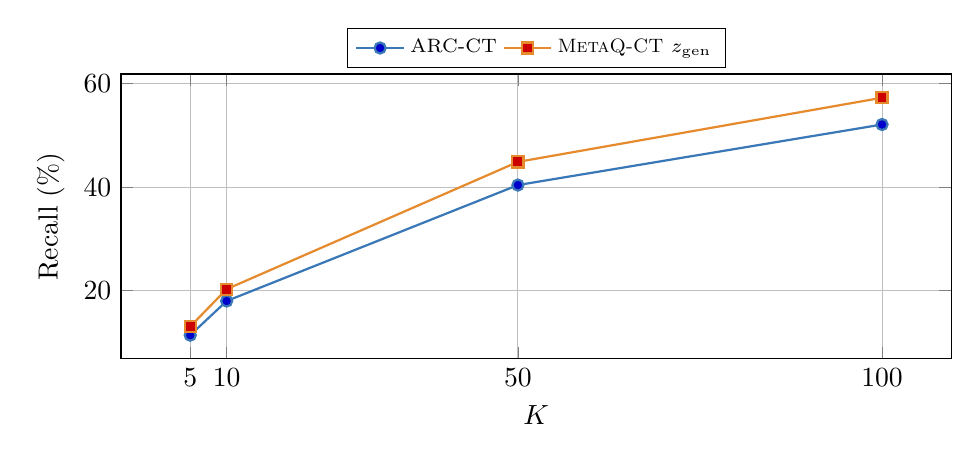
\begin{tikzpicture}
\begin{axis}[
  width=\columnwidth,height=5.2cm,
  xlabel={$K$},ylabel={Recall (\%)},
  xtick={5,10,50,100},grid=major,
  legend style={at={(0.5,1.02)},anchor=south,legend columns=2,font=\scriptsize}
]
\addplot+[mark=*,thick,color=ctblue] coordinates {(5,11.4)(10,18.0)(50,40.4)(100,52.1)};
\addplot+[mark=square*,thick,color=ctxorange] coordinates {(5,13.07)(10,20.29)(50,44.88)(100,57.27)};
\legend{ARC-CT,\ours{} $z_{\mathrm{gen}}$}
\end{axis}
\end{tikzpicture}
\caption{Canonical report-to-CT retrieval without retrieval-specific fitting.}
\label{fig:retrieval}
\end{figure}

\subsection{Preliminary report generation}
We attach a four-layer resampler and matched Qwen3-8B LoRA decoder to either
30 general tokens (CT-only) or all 49 adult C1 tokens. Both arms map to exactly
32 prefix tokens and optimize report teacher forcing plus an identical
class-balanced 18-label auxiliary loss. Metadata text is never supplied
directly to the language model.

The CT-only arm completed generation on 4,589 development studies, reaching
BLEU-1/2/3/4 of 0.4092/0.3202/0.2665/0.2309 and ROUGE-L of 0.4236. Its best
development loss is 0.53985. The recoverable C1 checkpoint is effectively tied
at 0.54004. We do not claim a C1 report-generation gain until correct, blank,
and shuffled-indication generations, F1-RadGraph, RadFact-CT, bootstrap
intervals, and blinded radiologist review are complete. These preliminary
values are intentionally excluded from the abstract's claims.

\section{Discussion}
The pediatric improvement is large, seed-consistent, positive across all 23
pathologies, and nearly eliminated by assigning the wrong indication. This
pattern supports a clinically plausible mechanism: detailed pediatric
indications provide pathology-specific prior information that is aligned with
the conditioned query design. The largest gains occur for pneumothorax,
pulmonary metastases, post-treatment change, pulmonary cysts, and mosaic
attenuation.

The adult result tells a different story. Correct, blank, and shuffled
indications yield 0.8781 and 0.8754 AUROC for the true and blanked arms on the
final checkpoint, with the shuffled arm not yet available. The full
architecture improves over CT-only, but the small intervention gap indicates
that adult CT-RATE indications are often missing or generic and that much of
the improvement arises from class-specific residual adaptation. We therefore
avoid attributing the entire adult gain to indication semantics.

Retrieval further clarifies which component contributes. The isolated general
bank retains a strong canonical embedding and achieves leading recall, whereas
post-hoc metadata mixing slightly degrades it. Metadata conditioning was
optimized for class-specific diagnosis rather than global report alignment. A
retrieval-specific conditioned contrastive objective is needed before claiming
metadata-aware retrieval improvement.

\section{Limitations}
The pediatric cohort is retrospective and single-institutional. The historical
1,507-case score was obtained on the Stage-2 model-selection validation cohort,
not an independent final test, and is therefore labeled validation throughout.
The new MRN-disjoint $<18$ protocol reduces this ambiguity, but its source test
pool was visible in earlier exploratory analyses. The age-$\geq5$
experiment changes both cohort and target schema relative to earlier all-age
work, so it does not establish that younger children corrupt training. A
factorial all-age versus age-$\geq5$ comparison with the same 23 labels is
required. Every pediatric comparison row is a local measurement rather than a
published external benchmark, and several are not architecture-matched: the
BiomedCLIP rows apply a 2-D encoder slice-wise with no volumetric context, the
Merlin row transfers an abdominal model, and the two probe rows use supervised
linear heads rather than prompt inference. Four further methods reported on
adult CT-RATE (BIUD, ViSD-Boost, BrgSA, and fVLM) could not be measured at all
because their releases lack code, weights, training entry points, or a
license. We state this rather than importing their adult figures into a
pediatric table. A pediatric CT-CLIP fine-tune also remains outstanding, since
its preprocessing cache exceeded available scratch quota. Only its zero-shot
transfer is reported. The strongest supervised CT-RATE result
comes from a separate single-checkpoint implementation and needs multi-seed
replication. Direct RAD-ChestCT transfer remains below the strongest published
baselines. Finally, report-generation clinical metrics and radiologist review
are not yet complete.

\section{Conclusion}
On historical held-out validation, pathology-specific conditioning of a
volumetric CT Q-Former with indication, age, and sex produces a reproducible
4.63-point pediatric macro-AUROC gain and
a 2.09-point adult CT-RATE gain over matched CT-only models. Counterfactual
inference shows that the pediatric improvement depends strongly on the correct
clinical indication. The model also preserves a strong general representation
for cross-modal retrieval. Together, these findings motivate clinical context
as an explicit, auditable component of volumetric medical vision--language
models.

\appendix
\section{Complete Per-Class Results}

\begin{table*}[t]
\centering
\caption{Pediatric age-$\geq5$ per-class AUROC, averaged over three seeds.}
\label{tab:pedsclass}
\begin{tabular}{@{}lrrr@{\hspace{1.0cm}}lrrr@{}}
\toprule
Pathology & CT-only & C1 & $\Delta$ & Pathology & CT-only & C1 & $\Delta$ \\
\midrule
Medical material & .8562 & .9024 & +.0463 & Peribronchial thickening & .8236 & .8431 & +.0195 \\
Cardiomegaly & .9441 & .9528 & +.0088 & Consolidation & .9241 & .9286 & +.0045 \\
Pericardial effusion & .7880 & .8125 & +.0245 & Bronchiectasis & .9101 & .9250 & +.0149 \\
Lymphadenopathy & .8042 & .8163 & +.0121 & Interlobular septal thickening & .8462 & .8828 & +.0366 \\
Atelectasis & .7126 & .7233 & +.0107 & Post-surgical/treatment change & .7485 & .8658 & +.1174 \\
Lung nodule & .6507 & .6937 & +.0431 & Pulmonary metastases & .6662 & .8036 & +.1374 \\
Lung opacity & .8148 & .8329 & +.0181 & Tree-in-bud & .8280 & .8737 & +.0457 \\
Pulmonary fibrotic sequela & .7512 & .7764 & +.0252 & Pulmonary cyst & .7523 & .8548 & +.1025 \\
Pleural effusion & .9729 & .9754 & +.0025 & Mass/neoplasm & .8496 & .8680 & +.0184 \\
Mosaic attenuation & .7413 & .8368 & +.0956 & Mucus plugging & .8622 & .9014 & +.0392 \\
Pleural thickening/nodule & .6607 & .6819 & +.0212 & Bone abnormality & .5789 & .6348 & +.0559 \\
Pneumothorax & .7606 & .9245 & +.1639 & \textbf{Macro mean} & \textbf{.7933} & \textbf{.8396} & \textbf{+.0463} \\
\bottomrule
\end{tabular}
\end{table*}

\begin{table*}[t]
\centering
\caption{Adult CT-RATE per-class prompt AUROC, averaged over three seeds.}
\label{tab:adultclass}
\begin{tabular}{@{}lrrr@{\hspace{1.0cm}}lrrr@{}}
\toprule
Pathology & CT-only & C1 & $\Delta$ & Pathology & CT-only & C1 & $\Delta$ \\
\midrule
Medical material & .9159 & .9447 & +.0287 & Lung nodule & .7270 & .7383 & +.0113 \\
Arterial wall calcification & .9336 & .9421 & +.0085 & Lung opacity & .8680 & .8844 & +.0164 \\
Cardiomegaly & .9343 & .9364 & +.0021 & Pulmonary fibrotic sequela & .7020 & .7463 & +.0443 \\
Pericardial effusion & .8957 & .9040 & +.0083 & Pleural effusion & .9768 & .9725 & -.0042 \\
Coronary wall calcification & .9273 & .9381 & +.0109 & Mosaic attenuation & .8163 & .8954 & +.0790 \\
Hiatal hernia & .8159 & .8209 & +.0050 & Peribronchial thickening & .8148 & .8261 & +.0113 \\
Lymphadenopathy & .7786 & .7923 & +.0136 & Consolidation & .9285 & .9334 & +.0049 \\
Emphysema & .8113 & .8251 & +.0138 & Bronchiectasis & .7995 & .8242 & +.0247 \\
Atelectasis & .7967 & .8103 & +.0136 & Interlobular septal thickening & .8120 & .8951 & +.0831 \\
\multicolumn{4}{c}{} & \textbf{Macro mean} & \textbf{.8475} & \textbf{.8683} & \textbf{+.0209} \\
\bottomrule
\end{tabular}
\end{table*}

\section{Auxiliary Supervised Readout}
For completeness, the best separate Biltir \texttt{ctx\_cls} checkpoint reaches
0.88386 macro AUROC on all 3,002 CT-RATE validation studies and 0.88484 on the
1,464-study indication-present subset. Full-split per-class AUROCs are listed
in Table~\ref{tab:ctxclsclass}. This appendix is deliberately separate from the
prompt-based primary result.

\begin{table*}[t]
\centering
\caption{Per-class AUROC of the supervised \texttt{ctx\_cls} checkpoint.}
\label{tab:ctxclsclass}
\begin{tabular}{@{}lrr@{\hspace{1.4cm}}lrr@{}}
\toprule
Pathology & Full & Ind.-present & Pathology & Full & Ind.-present \\
\midrule
Medical material & .9443 & .9390 & Lung nodule & .8052 & .8037 \\
Arterial wall calcification & .9426 & .9423 & Lung opacity & .8909 & .9004 \\
Cardiomegaly & .9442 & .9374 & Pulmonary fibrotic sequela & .7742 & .7831 \\
Pericardial effusion & .9287 & .9398 & Pleural effusion & .9767 & .9719 \\
Coronary wall calcification & .9460 & .9354 & Mosaic attenuation & .9135 & .9149 \\
Hiatal hernia & .8519 & .8707 & Peribronchial thickening & .8316 & .8165 \\
Lymphadenopathy & .7998 & .7867 & Consolidation & .9263 & .9338 \\
Emphysema & .8420 & .8310 & Bronchiectasis & .8553 & .8518 \\
Atelectasis & .8359 & .8540 & Interlobular septal thickening & .9005 & .9147 \\
\midrule
\multicolumn{3}{c}{} & \textbf{Macro mean} & \textbf{.88386} & \textbf{.88484} \\
\bottomrule
\end{tabular}
\end{table*}

\bibliographystyle{plain}
\bibliography{references}

\end{document}
